\documentclass[12pt]{extarticle}
\usepackage{geometry}
\usepackage{graphicx}
\usepackage{listings}
\usepackage{hyperref}
\usepackage[dvipsnames]{xcolor} % usato per i listati di codice più carini e coccolosi
\usepackage[italian]{babel}
\usepackage[utf8]{inputenc}
\usepackage[T1]{fontenc}

% impostazioni generali
\geometry{
	a4paper,
	top = 2cm,
	left = 2.5cm,
	bottom = 2cm,
	right = 2.5cm,
}
\lstset{
    language=C, 
    %frame=shadowbox,
    %rulesepcolor=\color{gray!50},
    basicstyle=\ttfamily\small,
    keywordstyle=\color{purple}\bfseries\small,
    stringstyle=\color{ForestGreen}\small,
    commentstyle=\color{blue}\small,
    numbers=left,
    numberstyle=\small\color{black},
    numbersep=5pt,
    tabsize=2,
    showtabs=false,
    showspaces=false,
    showstringspaces=false,
    %escapechar=|,
    %captionpos=b,
    breaklines=true,
    keepspaces=true
}

\author{Pierciro Caliandro (matr 0299815)}
\title{Report dell'homework \#4}
\date{}

\begin{document}
\maketitle
\section{Introduzione}
Il seguente documento riporta i passi analitici seguiti e le informazioni raccolte per quanto riguarda lo studio del programma \textbf{hw4.exe}.\\Tale eseguibile è un malware, quindi è stato analizzato prestando particolare attenzione all'ambiente di esecuzione, per evitare che quest'ultimo potesse subire dei danni gravi.\\L'obiettivo dell'analisi è quello di \textbf{trovare quante più informazioni possibili sull'eseguibile}, per cercare di capirne il funzionamento generale.
\section{Primo lancio dell'eseguibile}
Il programma viene fornito in formato compresso e andandolo ad estrarre dall'archivio, se non si disattivano tutte le protezioni fornite da Windows Defender, questo riconosce che il programma è un malware di tipo ransomware ed in particolare lo classifica come \textbf{LockyA}.\\Disabilitando il Defender ed eseguendo ugualmente il programma, in una VM apposita, questo gira per alcuni minuti ed infine mostra una serie di messaggi che informano l'utente che tutti i suoi file sono stati cifrati mediante l'utilizzo degli algoritmi di cifratura RSA-2048 e AES-128, indicando poi una serie di istruzioni necessarie per poter ottenere la chiave segreta usata per la cifratura e riavere indietro i propri dati.\\Anche lo sfondo del Desktop viene modificato, usando un immagine che riassume nuovamente le regole per poter riavere i propri file.\\Inoltre, all'interno di ogni cartella in cui il ransomware ha trovato dei file da cifrare, è presente il risultato della cifratura, che è un file con estensione ".asasin" così come anche un file con estensione .htm che riassume nuovamente le regole per poter ottenere il riscatto.  
\section{Unpacking dell'eseguibile}
La prima operazione effettuata è stata l'analisi statica di base dell'eseguibile. Usando il comando \texttt{file}, mediante shell di Linux, l'output restituito indica che il file è un eseguibile Windows a 32 bit (PE32), che sembra essere stato compresso con il programma UPX.\\Il file è stato quindi decompresso usando il comando \texttt{upx -d}, ma il programma ottenuto ha una taglia più o meno simile a quella del programma impacchettato.\\Si è quindi tentanto di effettuare anche uno spacchettamento manuale: aprendo infatti in OllyDbg il file impacchettato, la prima istruzione è una \texttt{PUSHAD}, che serve proprio per salvare tutti i registri sullo stack e procedere con l'unpacking del programma. È stato messo un breakpoint hardware sull'accesso ai dati presenti sullo stack, che ha permesso di arrivare fino alla \texttt{POPAD}, dopo la quale avviene il jump all'OEP (ad indirizzo 0040ea13).\\Si ottiene quindi un processo dumpato che ha una taglia leggermente maggiore di ciò che si ottiene semplicemente tramite la decompressione mediante UPX, ma nessuna delle euristiche utilizzate dal plugin OllyDump di OllyDbg permette di ottenere la Import Address Table.\\Utilizzando nuovamente il comando \texttt{file}, il nuovo eseguibile ottenuto risulta ancora compresso con UPX, quindi in realtà il processo ottenuto a seguito del dump va ulteriormente manipolato, inoltre se questa volta si prova a decomprimerlo con UPX stesso, il programma informa che il binario non risulta compresso con UPX.\\Si è quindi tornati ad eseguire il programma con OllyDbg:
\begin{itemize}
    \item La prima API invocata è la \texttt{IsBadStringPtrW}, la quale verifica se il processo corrente ha accesso in lettura a uno specifico range di memoria. La funzione prende due parametri, un puntatore a una stringa non nulla e un intero, che specifica il massimo numero di byte per cui la funzione verifica se vi è accesso in lettura. Il valore ritornato è quindi 0 se vi è accesso a tutti i byte fino al terminatore di stringa o fino al massimo specificato dal secondo parametro.\\Questa API viene invocata diverse volte, per verificare diverse aree di memoria 
    \item si arriva poi all'istruzione ad indirizzo 004069da, \texttt{CALL EBX}, che porta in una zona di indirizzi che, in base alle diverse run effettuate, presenta indirizzi che hanno i byte 5 e 6 (a partire da sinistra) ogni volta differenti
\end{itemize}
Vi sono poi due cicli interessanti:
un ciclo a partire dall'indirizzo 00**001d che esegue le istruzioni sottostanti:
\begin{itemize}
    \item \texttt{LODS DWORD PTR DS:[ESI]}
    \item \texttt{CALL 00**30ef}
    \item \texttt{MOV DWORD PTR DS:[ESI-4], EAX}: consultando i registri di OllyDbg, è possibile vedere che viene caricata, ad ogni iterazione del ciclo, una diversa funzione di libreria
    \item \texttt{LOOPD SHORT 00**001d}
\end{itemize}   
L'altro ciclo invece comincia dall'indirizzo 00**00dc, dove vengono ogni volta caricate informazioni relative alle sezioni del programma. In particolare, in ogni iterazione del ciclo, vengono caricate le stringhe ASCII nel registro EDI:
\begin{itemize}
    \item .text
    \item .rdata
    \item .data
    \item .reloc 
    \item .cdata
\end{itemize}
Si arriva infine ad un "long jump" in quanto ad indirizzo 00**01BE viene eseguita una \texttt{JMP ESI} che porta all'indirizzo 00402d8f.\\C'è poi una \texttt{CALL} alla funzione \texttt{FUN\_00406838}, prima della quale è stato preso un dump che ha permesso di vedere le DLL usate dal programma, seguita da un JUMP all'indirizzo 00402c22.\\Il processo ottenuto a seguito di questo dump, usando la 2° euristica del plugin "OllyDump" di OllyDbg ha permesso di ricostruire la IAT, quindi tale programma risultante è stato importato in Ghidra per poter proseguire l'analisi utilizzando in simultanea sia il disassembler che il debugger.\\L'entrypoint considerato si trova quindi ad indirizzo 00402d8f.\\

\section{Analisi del \texttt{main}}
Il main del programma considerato è l'ultima funzione chiamata dentro l'entrypoint, ad indirizzo 0042c820.\\La prima CALL incontrata è alla API \texttt{GetModuleHandleA}, a cui viene passato come parametro una stringa \texttt{NULL}: questo ha l'effetto di restituire un handle al file .exe usato per creare questo programma. Vengono poi messi sullo stack i valori 89000 ed il contenuto di EAX, ovvero l'handle alla funzione precedente, per poi passare alla CALL della funzione \texttt{FUN\_00477050}

\subsection{Analisi della \texttt{FUN\_00477050}}
Inizialmente vi è un \texttt{while(true)}, che viene superato mettendo un breakpoint sull'istruzione successiva.\\Vi è quindi la \texttt{CALL} all'API \texttt{VirtualAlloc}:
\begin{itemize}
    \item l'API manipola una certa regione dello spazio di indirizzamento virtuale del processo
    \item il primo parametro è l'indirizzo iniziale della zona di memoria da allocare, ed essendo in questo caso passato pari a \texttt{NULL}, tale zona viene scelta dal sistema operativo
    \item il secondo parametro è la taglia, in byte, della memoria che viene allocata
    \item viene poi passato come 4° parametro un flag che permette alle pagine di essere accedute in read/write mode
\end{itemize}
Il valore di ritorno è l'indirizzo di base della zona allocata, che viene poi salvata ad indirizzo dato da EBP -0x8.\\Andando avanti, ad indirizzo 00477573 vi è l'accesso al segmento FS, ad offset 18h arrivando quindi alla TEB: la TEB viene poi messa in EAX e successivamente si fa una \texttt{MOV EAX, DWORD PTR[EAX + 0x30]} e ad offset 30 della TEB c'è la struttura PEB del processo.\\Più avanti, ad indirizzo 004774be c'è una \texttt{MOVZX} in EAX spiazzandosi a offset 2 della PEB, quindi si carica nel registro il valore del campo \texttt{BeingDebugged} della PEB: difatti in seguito all'istruzione, nel registro \texttt{EAX} vi è il valore 1 (che indica la presenza di un debugger).\\Siccome tale sequenza di istruzioni può essere usata per realizzare un meccanismo anti-debugging, in quanto il valore di EAX viene poi successivamente verificato, è stata introdotta una patch al binario andando a sostituire l'operazione di \texttt{MOVZX} con le seguenti istruzioni:
\begin{itemize}
    \item \texttt{XOR EAX,EAX}
    \item \texttt{NOP}
    \item \texttt{NOP}
\end{itemize}
A questo punto, si eseguono una serie di operazioni che avvengono in un ciclo \texttt{while}, che prosegue finché non è stata raggiunta la taglia della regione di memoria allocata.\\Completato il ciclo, viene nuovamente invocata la \texttt{VirtualAlloc}, con gli stessi parametri di prima ma questa volta richiedendo di allocare memoria per un totale di byte pari a 0x6494, dimensione ottenuta in seguito alle operazioni svolte in precedenza.\\Viene successivamente invocata la \texttt{VirtualFree}, dopo aver effettuato altre operazioni sulla regione di memoria allocata per prima, che va a liberare tale memoria allocata (che iniziava ad indirizzo 00540000), dopo di che il controllo ritorna al \texttt{main}.\\È stata quindi analizzata la seconda funzione invocata dal \texttt{main}, la \texttt{FUN\_00429ea0}.


\subsection{Analisi della \texttt{FUN\_00429ea0}}
Nella funzione, ad indirizzo 0042c17b viene invocata l'API \texttt{SetErrorMode}: viene passato come parametro 0x8003 e tale combinazione dei possibili flag fa si che vengano mascherati all'utente determinati errori del programma, in particolare evita che vengano mostrati degli error box per errori dovuti a
\begin{itemize}
    \item funzione \texttt{OpenFile} che fallisce in quanto non viene trovato il file da aprire
    \item non viene mostrato un errore critici
    \item non viene mostrato il Windows Error dialogue box 
\end{itemize}
Successivamente, c'è la chiamata alla \texttt{SetUnhandledExceptionFilter}: questa API imposta un handler che verrà chiamata quando il processo non riesce a gestire delle eccezioni, se il processo non è debuggato.\\Viene passato come parametro l'indirizzo alla funzione da invocare che verrà invocato quando la funzione \texttt{UnhandledExceptionFilter} prenderà il controllo ed il processo non sarà debuggato.\\Tale funzione passata come parametro è ad indirizzo 0041f820 ed è stata rinominata come \texttt{handle\_exception}\\Vi è in segutio l'invocazione della \texttt{FUN\_0042cf00}

\paragraph{Analisi della \texttt{FUN\_0042cf00}}
All'indirizzo  0042cf0c c'è una chiamata alla \texttt{GetCurrentProcess}: tale API restituisce uno pseudo-handle al processo corrente e questo handle viene passato come parametro alla CALL verso la \texttt{LAB\_0047a058}, che risulta essere l'API \texttt{OpenProcessToken}:
\begin{itemize}
    \item la funzone apre il token di accesso associato al processo
    \item il primo parametro è un handle al processo mentre il secondo costituisce i diritti di accesso, passati in questo caso come \texttt{TOKEN\_ADJUST\_DEFAULT}
    \item nel terzo parametro viene restituito un puntatore all'handle verso il nuovo token di accesso aperto.
\end{itemize}
Se l'operazione ha successo viene invocata la \texttt{SetTokenInformation} che va ad impostare delle informazioni per il token d'accesso, in base ai parametri passati viene richiesto di disabilitare la virtualizzazione.\\La funzione termina chiudendo l'handle precedentemente recuperato.\\\\Andando avanti con l'analisi, si arriva alla CALL di 3 API, il cui valore di ritorno viene valutato all'interno di un if:
\begin{itemize}
    \item \texttt{GetSystemDefaultLangID}, la quale  restituisce l'identificativo del linguaggio del sistema; 
    \item \texttt{GetUserDefaultLangID}, che restituisce invece l'identificativo per il Region Format del linguaggio utente; 
    \item infine, la \texttt{GetUserDefaultUILanguage}, che fornisce in output l'identificatore per la UI dell'utente
\end{itemize}
I valori di ritorno della 3 API vengono confrontati in un predicato booleano che considera l'AND fra i risultati ed il cui risultato porta all'invocazione di una \texttt{Sleep}, che porta a dormire per 2ee0h = 12272ms. Al risveglio, si passa ad invocare la \texttt{FUN\_0041f680} 

\paragraph{Analisi della \texttt{FUN\_0041f680}}
All'interno della funzione avviene quanto segue:
\begin{itemize}
    \item vi è la CALL a \texttt{GetModuleFileNameW}: l'API  recupera il path completo del file contenente il modulo che viene richiesto,  prende 3 parametri:
    \begin{itemize}
        \item \texttt{HMODULE}: handle al modulo di cui si richiede il path. In questo caso è \texttt{NULL}, quindi si richiede il path del file eseguibile corrente;
        \item puntatore ad un buffer che riceverà il path del modulo
        \item taglia del buffer di destinazione
    \end{itemize}
\end{itemize}
Difatti, in seguito alla chiamata, il buffer contiene proprio il path completo (a partire da "C:$\backslash$") del file eseguibile corrente.\\\\Si ritorna dalla funzione, per invocare la \texttt{FUN\_0041f560}: dentro la funzione si chiama l'API \texttt{GetTempPathW} che però come nel caso precedente, restituisce un output che non viene usato per tanto l'analisi procede senza approfondire.\\Si arriva in seguito all'invocazione della \texttt{FUN\_00431440}

\paragraph{Analisi della funzione \texttt{FUN\_00431440}} 
Vi è la chiamata alla \texttt{FUN\_0042f110}, che al suo interno invoca l'API \texttt{GetWindowsDirectoryA}: questa API recupera il percorso della cartella di Windows, che viene salvato nel buffer passato come primo parametro. Il valore di ritorno della funzione è infatti la stringa "C:$\backslash$Windows", proseguendo l'analisi vi è la CALL alla funzione \texttt{FUN\_004129f0} che effettua una copia del contenuto del primo parametro passato come input solamente se questo è diverso da \texttt{NULL} e se anche il secondo parametro passato in input è diverso da 0, in quanto di questo caso viene invocata una \texttt{memcpy}\\Si arriva poi ad invocare la \texttt{FUN\_0042f430}:
\begin{itemize}
    \item al suo interno la funzione chiama la \texttt{FUN\_0042f2e0} che a sua volta chiama l'API \texttt{GetVolumeNameForVolumeMountPointA}
    \item tale API fornisce il GUID path del volume fornito come primo parametro di input, in questo caso "C:$\backslash$Windows$\backslash$"
\end{itemize}
L'API fallisce, causando un'eccezione e restituendo come errore \texttt{ERROR\_NOT\_A\_REPARSE\_POINT}.\\Al ritorno dall'eccezione, il controllo torna alla chiamata della \texttt{FUN\_0042f430}, questa volta il parametro passato alla funzione è la stringa "C:$\backslash$", andando avanti con f8 in OllyDbg vi è come ultimo errore \texttt{ERROR\_MORE\_DATA}, ma ad indirizzo EBP + 0x1c vi è la stringa "$\backslash$$\backslash$?$\backslash$Volume\{a04afba1-0000-0000-0000100000000000\}".\\Tale valore viene poi copiato, dalla \texttt{FUN\_004203a0} nell'area di memoria ad indirizzo dato da EBP -0x38, vi sono poi una serie di funzioni il cui effetto globale sembra quello di manipolare la stringa precedente, lasciando in EBP -0x38 "\{a04afba1-0000-0000-0000100000000000\}".\\Vi è in seguito interazione con funzioni che eseguono operazioni crittografiche:
\begin{itemize}
    \item la \texttt{FUN\_00416570} invoca al suo interno la \texttt{CryptAcquireContextA}:
    \begin{itemize}
        \item questa API è usata per acquisire un handle ad un container di chiavi all'interno di uno specifico Cryptographic Service Provider, che è un modulo software che esegue algoritmi crittografici per autenticazione, cifratura ed encoding.
        \item il primo parametro riceve l'handle al CSP
        \item essendo il secondo ed il terzo parametro sono passati \texttt{NULL}, dalla documentazione questo implica che viene richiesto di utilizzare il CSP di default
    \end{itemize}
    \item vi è poi la chiamata della \texttt{FUN\_0042cb70} che invoca al suo interno la \texttt{CryptCreateHash}: 
    \begin{itemize}
        \item tale API inizializza l'hashing di uno stream di dati, restituendo al chiamante un handle ad un oggetto hash.
        \item in base ai parametri di input, viene creato un oggetto hash su cui verrà usato l'algoritmo MD5, l'handle a tale oggetto è in EBP -0x18
    \end{itemize}
    \item successivamente, si invoca la \texttt{FUN\_0042cdd0}, dove viene invocata la \texttt{CryptHashData}:
    \begin{itemize}
        \item l'API aggiunge dei dati ad uno specifico hash object, in questo caso quello aperto in precedenza
        \item i dati aggiunti sono proprio la stringa "\{a04afba1-0000-0000-0000100000000000\}"
    \end{itemize}
    \item proseguendo si arriva alla \texttt{FUN\_00430010}, che invoca \texttt{FUN\_0042fa00} la quale a sua volta invoca la \texttt{FUN\_0042ccb0}.\\Questa al suo interno chiama la API \texttt{CryptGetHashParam} che recupera i dati che governano le operazioni su un oggetto hash. I dati vengono restituiti nel 3° parametro, ad indirizzo EBP -0xac. C'è poi un ciclo while in cui si usa la stringa costante \texttt{0123456789ABCDEF}.\\ Il risultato è la stringa "1BCC0199BD4620BFEC62CC688612AB1C", che è quindi presumibilmente l'hash risultante dalla stringa precedente. Questo viene salvato nel buffer ad indirizzo EBP -0x8c.
    \item poi, viene chiamata la \texttt{FUN\_00420300} il cui effetto visibile è che viene tagliato l'hash precedente e copiato ad indirizzo EBP -0x70, che contiene infatti "1BCC0199BD4620BF"
    \item si invoca poi la \texttt{CryptDestroyHash}, che distrugge l'oggetto hash precedentemente copiato
    \item per concludere, si invoca la \texttt{CryptReleaseContext}, che rilascia l'handle al CSP.
\end{itemize}
Al ritorno dalla funzione, l'hash troncato è presente all'indirizzo EBP -0xfc.\\\\Viene poi chiamata la \texttt{FUN\_004203a0}, che copia la stringa suddetta dentro \texttt{DAT\_00481fb4}.\\La chiamata successiva alla \texttt{FUN\_00426a40}: 

\paragraph{Analisi della \texttt{FUN\_00426a40}}
Viene ripresa la stringa troncata dal dato \texttt{DAT\_00481fb4}, c'è poi un ciclo while dove viene generata una stringa a partire da quella precedente, che è "2aCaDa..." e a cui viene in seguito concatenata la stringa "$\backslash$Global" e poi la stringa "$\backslash$Local", entrambe in seguito alla chiamata della \texttt{FUN\_00420fc0}, la posizione in memoria per le stringhe concatenate è rispettivamente EBP -0x78 e EBP -0x58.\\Viene poi messo nel registro EDI l'API \texttt{OpenMutexA}, per effettuarne successivamente due CALL:
\begin{itemize}
    \item la prima CALL prende come primo parametro la stringa "Global", mentre la seconda "Local"
    \item entrambe le CALL falliscono, restituendo \texttt{NULL} ed errore \texttt{ERROR\_FILE\_NOT\_FOUND}
\end{itemize}
Successivamente, viene invocata due volte la \texttt{FUN\_0041a6a0}, assegnando il valore restituito da ognuna delle chiamate rispettivamente agli indirizzi \texttt{DAT\_004831f4} e \texttt{DAT\_00483200}

\subparagraph{Analisi della \texttt{FUN\_0041a6a0}}
Dopo aver impostato il valore di alcune variabili locali, viene invocata la \texttt{AllocateAndInitializeSid}: l'API alloca ed inizializza un Security Identifier (SID) con al più 8 sotto-autorità. In base ai parametri passati, viene richiesto di creare un SID con una sotto-autorità e la struttura di dati risultante verrà restituita nel puntatore alla variabile locale \texttt{local\_c}.\\Successivamente, viene invocata la \texttt{SetEntriesInAclA}
\begin{itemize}
    \item l'effetto è quello di creare una nuova ACL (Acess Control List) unendo nuove ACL oppure considerandone già esistenti
    \item in base ai parametri, viene passata una sola struttura di tipo \texttt{EXPLICIT\_ACCESS}, che contiene le informazioni riguardo l'AC e che verranno unite all'ACL già esistente
    \item essendo il 3° parametro NULL, la funzione crea una nuova ACL il cui pointer viene restituito nel 4° parametro
\end{itemize}
La funzione va a buon fine, e viene quindi invocata la \texttt{InitializeSecurityDescriptor}:
\begin{itemize}
    \item questa API inizializza un nuovo descrittore di sicurezza
    \item le informazioni di inizializzazione vengono scritte nel primo parametro passato alla funzione 
\end{itemize}
In seguito all'invocazione con successo di tale API, viene invocata la \texttt{SetSecurityDescriptorDacl}:
\begin{itemize}
    \item l'API imposta le informazioni di una ACL discrezionaria (DACL). Se la DACL esiste già nel SID passato come primo parametro, essa viene rimpiazzata
    \item siccome il 2° parametro è TRUE, viene inserita la DACL specificata dal 3° parametro, ovvero quella ottenuta dalla \texttt{SetEntriesInAclA}
\end{itemize}
Infine viene creato un nuovo oggetto evento mediante la \texttt{CreateEventA}, dove viene passata una struttura dati come primo parametro i cui primo campo, ovvero \texttt{lpSecurityDescriptor} è la DACL creata in precedenza, viene poi usato come nome dell'evento la stringa "Global$\backslash$2aCaDa...".\\Per concludere il SID precedentemente allocato viene chiuso e de-allocato invocando la \texttt{FreeSid}.\\\\
Una volta tornati dalla funzione, viene valutato il valore restituito in un if, dove viene anche considerato in OR il valore di ritorno della \texttt{FUN\_004270f0}\\

\subparagraph{Analisi della \texttt{FUN\_004270f0}}
Nella funzione, viene inizialmente invocata la \texttt{FUN\_00420fc0}, che scrive ad indirizzo EBP - 0x44 la stringa "$\textasciitilde$$\textasciitilde$$\textasciitilde$" seguita dalla stringa "1BCC0199BD4620BF".\\Vi è poi la chiamata della \texttt{FUN\_004211f0}, che concatena alla stringa precedente ancora la stringa "$\textasciitilde$$\textasciitilde$$\textasciitilde$", per copiare il risultato in EBP -0x28.\\Tale stringa viene poi passata come parametro alla \texttt{GlobalFindAtomA} che ricerca nella atom table globale il valore associato alla stringa.\\La API non trova la corrispondenza, quindi si effettua una ricerca nella atom table locale mediante la \texttt{FindAtomA}, nuovamente senza successo.\\\\Si ritorna nella \texttt{FUN\_00429ea0} e viene invocata la \texttt{FUN\_00423740}  

\paragraph{Analisi della \texttt{FUN\_00423740}}
Viene come prima cosa invocata la \texttt{FUN\_00420300} che restituisce la stringa precedentemente tagliata troncata ai 6 byte più significativi.\\Tale stringa viene poi passata alla funzione d libreria \texttt{\_strtoul}, successivamente viene di nuovo chiamata la \texttt{GetUserDefaultLangID}.\\C'è poi la CALL all'API \texttt{GetVersionExA}: questa API prende un solo parametro, di tipo \texttt{LPOSVERSIONINFOA}, e restituisce informazioni relativamente al SO host, dal codice è possibile vedere che il parametro passato in input è ad indirizzo dato da EBP - 0x100.\\In seguito, viene invocata la funzione \texttt{GetSystemMetrics} per recuperare delle informazioni relative a metriche di sistema o impostazioni di configurazione, viene passato il parametro "89" che quindi riceve informazioni diverse da 0 se il sistema operativo è WindowsServer 2003.\\Viene poi invocata la \texttt{FUN\_0042d1d0}:
\begin{itemize}
    \item viene invocata la \texttt{GetModuleHandleA} per recuperare l'handle associato al modulo "kernel32.dll"
    \item successivamente, viene invocata la \texttt{GetProcAddress} che restituisce l'indirizzo dell'API "IsWow64Process"
    \item viene poi chiamata la \texttt{GetCurrentProcess} per ottenere un handle al processo corrente, usato poi come primo parametro per la chiamata alla \texttt{IsWow64Process}, che determina l'architettura di processore su cui è in esecuzione il processo.
\end{itemize}
Al ritorno dalla \texttt{FUN\_0042d1d0}, viene invocata la \texttt{DsRoleGetPrimaryDomainInformation} che restituisce informazioni relativamente allo stato del computer. La funzione però fallisce, restituendo come errore \texttt{ERROR\_IO\_PENDING}.
\\\\Il valore restituito dalla funzione viene copiato in \texttt{DAT\_481fb4}\\Si prosegue poi all'interno di un ciclo \texttt{while}, dove è possibile vedere sullo stack in OllyDbg la stringa "html class='whlrmyq' data aqdmnub='uolyvvhd$>$$<$head$>$ $<$meta ch'", nel doppio \texttt{while(true)} viene quindi caricato e manipolato il codice di una pagina HTML.\\In seguito al ciclo, vi è l'invocazione della \texttt{FUN\_0046c640}

\paragraph{Analisi della \texttt{FUN\_0046c640}} La funzione parte azzerando determinati parametri sullo stack (spiazzandosi rispetto ad EBP), per poi invocare per 3 volte consecutive la \texttt{FUN\_0046c150}\\

\subparagraph{Analisi della \texttt{FUN\_0046c150}} La funzione è stata analizzata in quanto contenente delle chiamate a delle API che interagiscono con la rete. La prima di queste è la \texttt{WNetOpenEnumW}: questa API inizia l'enumerazione delle risorse di rete o delle connessioni aperte, che può essere proseguita chiamando la \texttt{WNetEnumResource}, in quanto viene restituito un handle nel 5° parametro passato alla funzione e che può essere utilizzato nelle chiamate successive.\\Viene quindi poi allocata memoria dinamica, salvata nella variabile locale \texttt{lpNetResource} per entrare in un ciclo \texttt{while(true)}:
\begin{itemize}
    \item viene invocata la \texttt{FUN\_00461200} che al suo interno invoca proprio la \texttt{WNetEnumResource}, che prosegue l'enumerazione iniziata precedentemente. Le informazioni trovate dalla funzione vengono restituite nel buffer di cui si passa il puntatore come terzo parametro, che è quindi un array di strutture di tipo \texttt{NETRESOURCE};
    \item al ritorno dalla \texttt{FUN\_00461200}, si verifica se il valore restituito è true, in tal caso si effettuano altri controlli su dei campi della struttura di dati recuperata, in particolare accedendo al campo \texttt{dwUsage} che restituisce una bitmask che da informazioni sull'usabilità della risorsa
    \item nel caso in cui non venga rispettato il primo controllo, si invoca la \texttt{WNetAddConnection2W}, che effettua una connessione ad una risorsa di rete. La risorsa viene specificata proprio dalla struttura \texttt{NETRESOURCE} precedentemente trovata, mentre username e password usate dipendono dal contesto utente.
\end{itemize}
La funzione termina, chiudendo l'handle tramite la \texttt{WNetCloseEnum} nel momento in cui viene restituito \texttt{false} dalla \texttt{FUN\_00461200}.\\\\Vi sono poi diverse chiamate ad API che interagiscono con i dischi:
\begin{itemize}
    \item \texttt{GetLogicalDrives}: restituisce una bitmask che rappresenta i dischi attualmente disponibili. In EAX a seguito della CALL c'è il valore 0x00000004; 
    \item la bitmask ottenuta viene quindi manipolata e verificata in un if, per ottenere la stringa UNICODE "c:$\backslash$" e viene in seguito passata come parametro alla \texttt{GetDriveTypeW}, in quanto la funzione richiede la directory root del drive.\\Il valore di ritorno della API è pari a 3, che indica che l'hard drive è di tipo fisso (hard disk o flash drive);
    \item viene poi verificato se il valore restituito dalla funzione è 4, quindi se il drive è remoto di rete, ma non essendo questo il caso si arriva a chiamare la \texttt{GetVolumeInformation}: l'API e fornisce informazioni sul file system ed il volume associati alla root directory, prende 8 parametri di cui il primo è il root path name, nuovamente passato come prima. L'altro parametro interessante che viene passato diverso da NULL è il 6°, che ottiene in output dei flag legati al volume ed al file system. 
\end{itemize}
Si torna dalla \texttt{FUN\_0046c640} e si prosegue, analizzando la \texttt{FUN\_00476b50}

\paragraph{Analisi della \texttt{FUN\_00476b50}}
La funzione al suo interno invoca la \texttt{FUN\_00474820}: questa funzione prende un solo parametro, di tipo stringa, ed effettua diverse chiamata ad API:
\begin{itemize}
    \item \texttt{GetCurrentProcess}: restituisce un pseudo-handle al processo corrente
    \item \texttt{OpenProcessToken}, che apre il token di accesso associato al processo di cui è stato passato l'handle
    \item \texttt{LookupPrivilegeValueA} che restituisce l'identificatore locale (LUID) usato sul sistema per rappresentare un determinato privilegio. Viene in questo caso richiesta l'informazione per il privilegio "SeDebugPrivilege" ed il LUID viene salvato nella variabile globale \texttt{DAT\_0048206c}
    \item viene in seguito invocata la \texttt{AdjustTokenPrivileges}, che va a abilitare o disabilitare privilegi relativi ad un determinato token di accesso.
    \item si accede infine a \texttt{GetLastError}, per verificare se tutti i valori sono stati modificati, cosa che è confermata dal fatto che il codice è ERROR\_SUCCESS
\end{itemize}
La funzione va quindi a cambiare le informazioni relative ad i privilegi del processo. Tale funzione viene chiamata per 4 volte, passando ogni volta una stringa diversa relativa ad un diverso privilegio:
\begin{itemize}
    \item "SeDebugPrivilege"
    \item "SeTakeOwnershipPrivilege"
    \item "SeBackupPrivilege"
    \item "SeRestorePrivilege"
\end{itemize}
Si passa quindi ad invocare la \texttt{GetModuleHandleA}, per ottenere un handle alla DLL "ntdll.dll", si invoca poi la \texttt{GetProcAddress} per ottenere l'indirizzo delle seguenti API:
\begin{itemize}
    \item "NtQuerySystemInformation", salvato in \texttt{DAT\_004831f0}
    \item "NtDuplicateObject", salvato in \texttt{DAT\_004831e8}
    \item "NtQueryObject", salvato in \texttt{DAT\_004831e}
\end{itemize}
Vi è poi una chiamata alla \texttt{CreateThread}: l'API crea un nuovo thread che esegue nell'address space virtuale del processo corrente.\\Prende 6 parametri 
\begin{itemize}
    \item[1] un puntatore ad una struttura di tipo \texttt{SECURITY\_ATTRIBUTES}, che determina se l'handle restituito può essere ereditato dai processi figli. In questo caso, essendo passato come \texttt{NULL}, questo non può avvenire;
    \item[2] taglia iniziale dello stack, pari a 0
    \item[3] routine che eseguirà il thread, ad indirizzo 004768d0
    \item[4] puntatore alla variabile da passare al thread, in questo caso \texttt{NULL} 
    \item[5] flag di creazione
    \item[6] thread id
\end{itemize}
Si torna quindi nuovamente nella \texttt{FUN\_00429ea0}\\\
Proseguendo l'analisi, vi è nuovamente la creazione di thread all'interno di un ciclo \texttt{for}, sempre mediante l'API \texttt{CreateThread}:
\begin{itemize}
    \item in questo caso, rispetto alla creazione precedente, la funzione che il thread deve eseguire è ad indirizzo 00429b40
    \item il parametro passato è l'indice usato nel ciclo for
\end{itemize}

L'handle al thread viene controllato (se pari a NULL o -1) per poi essere messo in EBP - 0x34, inoltre dall'esecuzione in OllyDbg viene creato un solo thread.\\Si prosegue quindi ad analizzare la \texttt{FUN\_0040fa10}

\paragraph{Analisi della \texttt{FUN\_0040fa10}} La prima funzione invocata è la \texttt{CoInitializeEx}, che si occupa di inizializzare la libreria COM, tale libreria viene usata per permettere la creazione di oggetti per effettuare la comunicazione fra processi.\\In seguito si passa ad invocare la \texttt{CoInitializeSecurity}, che imposta i valori di default per la sicurezza del processo corrente.\\Viene poi chiamata della \texttt{FUN\_00478420}:
\begin{itemize}
    \item viene chiamata la \texttt{LoadLibraryA}, passando come parametro la stringa "vssapi.dll". Viene restituito l'handle a tale libreria
    \item viene poi chiamata la \texttt{GetProcAddress} per due volte, per caricare le API \\ \texttt{CreateVssBackupComponentsInternal} e \\ \texttt{VssFreeSnapshotPropertiesInternal}
\end{itemize}
La funzione si occupa quindi del caricamento delle seguenti API dalla DLL.Da qui non è stato possibile proseguire, in quanto l'esecuzione nel debugger portava ad uno stallo dell'applicazione o al verificarsi di diverse eccezioni, quindi si l'analisi è tornata al processo chiamante.\\\\

Al ritorno dalla funzione, si entra in un ciclo for in cui viene invocata, ad ogni iterazione, l'API \texttt{WaitForSingleObject}: 
\begin{itemize}
    \item questa API attende che un determinato oggetto è nello stato segnalato oppure scade un time-out 
    \item i due parametri sono l'handle all'oggetto ed il time-out. In questo caso, il time-out è pari ad infinito, quindi la funzione ritornerà solo dopo che l'oggetto sarà segnalato.
\end{itemize}
L'analisi riprende da 0042a4ce, per andare ad eseguire la \texttt{FUN\_4273c0}

\paragraph{Analisi della \texttt{FUN\_4273c0}} Nella funzione, viene caricato il valore contenuto nel dato \texttt{DAT\_0047d138} (corrispondente alla stringa "$\textasciitilde$$\textasciitilde$$\textasciitilde$"), viene poi invocata la funzione \texttt{FUN\_420fc0} che restituisce dentro EBP-0x44 la stringa \texttt{"$\textasciitilde$$\textasciitilde$$\textasciitilde$Y8GRW8UYGJ161GEN"}.\\Successivamente viene invocata la \texttt{FUN\_4211f0} che come già analizzato concatena alla stringa passata come secondo parametro quella passata come 3°, per copiare il risultato nel buffer passato come 1° parametro. Si ottiene quindi la stringa \texttt{"$\textasciitilde$$\textasciitilde$$\textasciitilde$Y8GRW8UYGJ161GEN$\textasciitilde$$\textasciitilde$$\textasciitilde$"} che viene passata come parametro alla API \texttt{AddAtomA} che salva la stringa in una atom table e riceve un identificatore univoco a 16 bit per accedere a tale stringa; tale aggiunta viene fatta anche nella atom table globale.\\\\Proseguendo, si verifica se il \texttt{DAT\_00481ffc} e se il valore è diverso da 0 si chiama la \texttt{FUN\_425870}

\paragraph{Analisi della \texttt{FUN\_425870}} La funzione chiama come prima la \texttt{FUN\_00420a70} dentro cui si invoca l'API \texttt{SHGetFolderPathW}, che recupera il path di una cartella mediante il suo valore CSIDL. Tale path viene poi copiato all'interno del primo parametro passato alla funzione, che è ad indirizzo EBP -0x104 e tramite OllyDbg è possibile vedere che la stringa trovata è proprio "C:$\backslash$Users$\backslash$IEUser$\backslash$Desktop" che è quindi il path del Desktop della macchina.\\\\Viene poi copiata in ESI la stringa "asasin", presa dal dato globale \texttt{DAT\_47cbe0}, per poi caricare la stringa ".htm" ed invocare due volte la funzione \texttt{FUN\_0040f9b} che appende la stringa "asasin.htm" al path trovato prima, copiando in EBP -0xcc.\\Viene poi ripetuto lo stesso procedimento, copiando nel buffer EBP -0xb0 la stringa "C:$\backslash$Users$\backslash$IEUser$\backslash$Desktop$\backslash$asasin.bmp".\\La prima stringa viene passata alla \texttt{FUN\_0042e6b0} che al suo interno invoca la \texttt{FindFirstFileW} che restituisce un handle al file trovato tramite la query. La funzione verifica quindi se il file htm è già presente sul desktop, ed in base al valore di ritorno viene invocata o meno, dalla \texttt{FUN\_425870} la \texttt{FUN\_0042e7d0} che si occupa proprio di creare tale file.\\Viene ripetuto lo stesso procedimento col file .bmp.\\Proseguendo, viene spostata in EAX la stringa "Control Panel$\backslash$Desktop" che viene utilizzata nella \texttt{FUN\_00416290} come secondo parametro per la \texttt{RegOpenKeyExA}: la funzione apre un registry key, in questo caso la chiave è la \texttt{HKEY\_CURRENT\_USER}, viene richiesto di creare la sotto-chiave "Control Panel$\backslash$Desktop".\\In seguito, \texttt{WallpaperStyle} da EBP -0x30 in EAX, per invocare poi la \texttt{FUN\_004205a0}:
\begin{itemize}
    \item viene messo in EAX la stringa WallpaperStyle
    \item CALL della \texttt{FUN\_00416390}, dentro cui viene invocata la \texttt{RegSetValueEx} che utilizza l'handle restituito dalla API precedente, che era stato aperto specificando fra i permessi \texttt{KEY\_QUERY\_VALUE}. L'API recupera il tipo ed il dato del valore specificato, in questo caso è "WallpaperStyle", le informazioni vengono messe nel 5° parametro.
\end{itemize}
Viene poi richiamata una seconda volta, questa volta per chiedere informazioni sul valore "TileWallpaper".\\Viene in seguito invocata l'API \texttt{SystemParameterInfoW}: la funzione può essere usata per impostare o ottenere informazioni riguardo ai parametri di sistema. Viene in questo caso passata l'opzione \texttt{SPI\_SETDESKWALLPAPER}, che imposta lo sfondo usando la bitmap (file .bmp) precedentemente creato e passato qui come 3° parametro.\\Dopo di che, viene invocata due volte l'API \texttt{ShellExecuteW}, che esegue il comando \texttt{open} aprendo entrambe i file .htm e .bmp, infine viene invocata la \texttt{RegCloseKey} per chiudere la chiave di sistema precedentemente aperta.\\\\Dopo aver fatto ciò, il programma salta fino all'indirizzo \texttt{0042c1a9}, dove viene invocata la \texttt{FUN\_431de0}

\paragraph{Analisi della \texttt{FUN\_431de0}} Si trova come prima CALL la funzione \texttt{FUN\_0041f680}, che invoca a sua volta la \texttt{GetModuleFileNameW} che ricevendo come primo parametro un handle \texttt{NULL}, restituisce il percorso del file eseguibile corrente, mettendolo nel buffer passato come 2° parametro (la stringa viene copiata in diversi punti dello stack, come ad esempio EBP -0x60).\\Subito dopo, si chiama la \texttt{FUN\_0041f560} che invoca la API \texttt{GetTempFileW}, che restituisce il path della directory designata a contenere i file temporanei, ovvero \\"C:$\backslash$Users$\backslash$IEUser$\backslash$AppData$\backslash$Local\\$\backslash$Temp$\backslash$", salvata in un buffer a EBP -0x98.\\Viene in seguito invocata la \texttt{SetFileAttributesW} che imposta gli attributi del file eseguibile impostando l'attributo \texttt{FILE\_ATTRIBUTES\_NORMAL}.\\Vi è poi l'invocazione della \texttt{FUN\_0042F4b0}, a cui vengono passati il puntatore ad indirizzo EBP -x014, il path delle cartelle temporanee, la stringa "sys" ed invoca al suo interno la \texttt{GetTempFileNameW}: l'API crea un file con nome temporaneo all'interno della cartella "Temp", aggiungendo il prefisso "sys" ed il file risultante è quindi "sysE5CE.tmp", scritto nel buffer ad EBP -x07C.\\Viene poi chiamata la \texttt{MoveFileExW}: l'API copia il file eseguibile "hw4.exe" nel nuovo path, passando come opzioni 9, quindi \texttt{MOVEFILE\_REPLACE\_EXISTING} + \texttt{MOVEFILE\_WRITE\_THROUGH}.\\Viene poi nuovamente invocata la \texttt{MoveFileExW}, passando come primo parametro il path del file temporaneo, NULL come secondo parametro e 4 come flag; dati i parametri passati, l'effetto è quello di far si che il file venga cancellato nel momento in cui il sistema viene riavviato.\\Viene poi messa sullo stack la stringa "cmd.exe /C del /Q /F" per invocare poi la \texttt{FUN\_0042fe10} in seguito alla quale sullo stack, ad indirizzo EBP -0x7C vi è la stringa precedente concatenata col path assoluto del file temporaneo. Successivamente viene invocata la \texttt{FUN\_00412c20}, che sposta la stringa in EBP -0xc0, per chiamare infine la \texttt{FUN\_0042ec10}

\subparagraph{Analisi della \texttt{FUN\_0042ec10}} Viene internamente invocata la \texttt{CreateProcessW}: la funzione crea un nuovo processo, il primo parametro è pari a NULL e quindi l'applicazione da lanciare è il primo token separato da spazio presente nel secondo parametro, ovvero il comando "cmd.exe". Il resto della stringa passata come secondo parametro sono quindi gli argomenti del programma che viene lanciato: 
\begin{itemize}
    \item \texttt{/C} fa si che il resto della stringa del comando vengano mantenute solo se sono rispettate determinate condizioni
    \item \texttt{del} è un comando che elimina uno o più file. Passando l'opzione \texttt{/F} viene richiesto di effettuare la cancellazione forzata di un file, mentre con \texttt{/Q} si specifica che la modalità del comando non è interattiva, ovvero non viene richiesta la conferma della cancellazione.
\end{itemize}
Con il comando si richiede quindi di cancellare il file eseguibile dalla cartella dove è stato originariamente aperto, inoltre nei flags viene richiesto che il processo abbia una nuova console e appartenga alla classe di priorità \texttt{IDLE\_PRIORITY\_CLASS}.\\\\All'uscita dalla funzione, si esegue l'epilogo ed il malware termina la sua esecuzione invocando la \texttt{ExitProcess(0)}
\\\\L'analisi è si è quindi spostata sui 2 thread generati, quindi sono stati messi due breakpoint per entrare nell'esecuzione dei due thread che vengono creati, per analizzarne il contenuto.


\section{Analisi dei due thread creati}
\subsection{Analisi del thread 1 (indirizzo 004768d)}
Il thread è composto da poche righe di codice, che realizzano un ciclo \texttt{do/while(true)}, dentro cui viene chiamata la \texttt{FUN\_00476150}
\paragraph{Analisi della \texttt{FUN\_00476150}} Viene invocata la \texttt{GetModuleFileNameA}, che restituisce il path del file che contiene il modulo specificato dall'handle che è il primo parametro, ovvero la variabile globale \texttt{DAT\_004831c8}.\\La stringa recuperata è "C:$\backslash$Windows$\backslash$SYSTEM32$\backslash$ntdll.dll" e viene passata come primo parametro alla \texttt{CreateFileA}: la funzione crea o apre un file di I/O, e prende i seguenti parametri:
\begin{itemize}
    \item[1] nome del file da aprire o creare, specificandone il path completo
    \item[2] accesso richiesto al file, in questo caso \texttt{GENERIC\_READ}
    \item[3] sharing mode, con valore \texttt{FILE\_SHARE\_READ} in questo caso
    \item[4] security attributes, passato come \texttt{NULL}
    \item[5] l'azione da prendere su un file o device che esiste o meno, con valore in questo caso \texttt{OPEN\_EXISTING} quindi il file viene aperto solo se esiste 
    \item[6] flag e attributi, pari a 0
    \item[7] handle ad un file di template, che viene passato \texttt{NULL}
\end{itemize}
La funzione restituisce, in caso di successo, un handle al file.\\\\Viene in seguito allocata della memoria mediante delle funzioni di libreria di Visual Studio, per poi invocare la \texttt{GetCurrentProcessId}, che recupera l'identificatore del processo corrente.\\Dopo aver fatto dei controlli sulla memoria allocata, si entra all'interno di un while, dove vengono invocate una serie di funzioni
\paragraph{Analisi della \texttt{FUN\_00474c30}} La funzione prende 3 parametri, due interni ed il carattere terminatore di stringa '$\backslash$0'.Viene chiamata la \texttt{OpenProcess}: l'API apre un oggetto processo locale, prende 3 parametri:
\begin{itemize}
    \item l'accesso all'oggetto, passato con valore 0x40 che richiede quindi di duplicare l'handle
    \item un booleano che se pari a true rende l'handle ereditabile, in questo caso è false
    \item process id, identificatore del processo da aprire. In questo caso, è il primo parametro passato come input alla funzione
\end{itemize}
La chiamata restituisce \texttt{NULL}, quindi l'apertura fallisce (viene restituito l'errore \texttt{ERROR\_ACCESS\_DENIED}) e quindi la funzione termina semplicemente restituendo 0.\\Tale condizione di ritorno viene messa in AND con il valore di ritorno della funzione \texttt{FUN\_4750e0}, quindi è stato messo un breakpoint sulla chiamata alla \texttt{FUN\_4750e0} per poterne analizzare il contenuto.
\paragraph{Analisi della \texttt{FUN\_4750e0}} Nella funzione, c'è un predicato booleano complesso, che considera fra le diverse condizioni, il valore di ritorno dell'API \texttt{CreateEventA}: l'API crea o apre un oggetto di tipo evento, con o senza nome e prende 4 parametri:
\begin{itemize}
    \item[1] attributi di sicurezza, un puntatore ad una struttura di tipo \texttt{LPSECURITY\_ATTRIBUTES}. Essendo passata come \texttt{NULL}, l'handle non è ereditabile
    \item[2] parametro con valore false che fa si che la funzione crei un oggetto evento di auto-reset
    \item[3] stato iniziale, in questo caso false e quindi non segnalato
    \item[4] nome dell'oggetto evento, passato come \texttt{NULL} e quindi viene creato un oggetto senza nome
\end{itemize}
Vengono effettuate due chiamate a tale funzione e gli handle risultanti vengono assegnati alle due variabili globali \texttt{DAT\_4831cc} e \texttt{DAT\_4831d0}. A seguito di una verifica sul valore della variabile globale \texttt{DAT\_4831d4}, si chiama la \texttt{CreateThread}: viene quindi creato un 3° thread, che prende come parametro proprio il \texttt{DAT\_4831d4}, quindi l'handle al secondo evento creato, mentre la routine da eseguire è la \texttt{LAB\_474ed0}.\\L'handle del nuovo thread creato viene salvato nella variabile globale \texttt{DAT\_004831d4}, per poi chiamare l'API \texttt{WaitForSingleObject}: questa API è già stata incontrata in precedenza, ed attende che l'oggetto di cui viene specificato l'handle, in questo caso l'evento creato, transiti nello stato segnalato.\\In seguito, viene invocata la \texttt{SetEvent}: tale funzione imposta l'oggetto specificato nello stato segnalato, l'unico parametro della funzione è l'handle all'oggetto evento, che è in questo caso la variabile \texttt{DAT\_00481cc}, ovvero l'handle del primo evento creato e passato come parametro al thread creato dalla funzione. Viene poi nuovamente chiamata la \texttt{WaitForSingleObject}, passando sempre l'handle al secondo evento, ma con un time-out di 200ms. Questa volta la funzione ritorna per via del fatto che il time-out è scaduto e l'oggetto non è nello stato signaled (valore 0x102L), dopo questa chiamata si verifica che il valore di ritorno non sia 0 ed in tal caso si procede con l'invocazione dell'API \texttt{TerminateThread}: vengono passati l'handle al thread da chiudere ed il codice di uscita del thread, pari a 0504.\\Infine, viene chiuso l'handle del thread e la funzione termina. Nella funzione si accede a diverse variabili globali vicine da un punto di vista di indirizzi, che vengono utilizzate ad esempio come parametro per il thread creato ed anche per impostare il loro valore con quello dei parametri presi dalla funzione.\\\\Al ritorno dalla funzione, il valore restituito viene valutato in un if, insieme anche al valore della \texttt{FUN\_00474c30} e nel caso in cui siano rispettate entrambe le condizioni (in AND), si chiama la \texttt{FUN\_00475540}, è stato quindi messo un breakpoint sull'istruzione di CALL per analizzare il contenuto di tale funzione.  
\paragraph{Analisi della \texttt{FUN\_00475540}} Nella funzione, dopo aver imposta il valore di diverse variabili locali, vi è la chiamata di una funzione di libreria \texttt{\_wcsnicmp}, che effettua il confronto fra due stringhe per un certo numero di caratteri specificati. Le due istanze di stringhe viste sono
\begin{itemize}
    \item "$\backslash$Device$\backslash$HarddiskVolume1$\backslash$Windows$\backslash$System32".\\Tale stringa era presente nel registro ESI già prima dell'invocazione della funzione ed è proprio il contenuto del buffer restituito dal thread 3 in seguito alla query.
    \item "$\backslash$Device$\backslash$mup" 
\end{itemize}
 e viene richiesto di confrontare 12 caratteri.\\Si verifica quindi il valore di ritorno, ed essendo diverso da 0 si arriva a richiamare la funzione che questa volta prende come secondo parametro la stringa "$\backslash$Device$\backslash$LanmanRedirector$\backslash$".\\In questo caso, se il valore di ritorno è diverso da 0, viene chiamata la \texttt{GetLogicalDriveStringsW}, che riempie il buffer passato come secondo parametro con stringhe che specificano dei dispositivi validi nel sistema.\\Viene passato un buffer di 3 caratteri, la stringa recuperata coincide col disco C del sistema, essendo "C:".\\Viene poi chiamata l'API \texttt{QueryDosDeviceW} che recupera le informazioni relative al nome di un device MS-DOS. Il primo parametro è il device MS-DOS su cui effettuare la query, in questo caso "C:", viene poi passato un puntatore al buffer che riceverà il risultato della query ed il numero massimo di caratteri che è possibile salvare nel buffer.\\Anche in questo caso si verifica se la funzione ha avuto successo, in tal caso si carica in EAX la prima strina recuperata dalla funzione, ovvero "$\backslash$Device$\backslash$HarddiskVolume1" e si cerca di verificare se fra le stringhe recuperate dall'ultima chiamata da API ce n'è una che corrisponde a quella contenuta in ESI.


\subsection{Analisi del thread 3 (indirizzo 00474ed0)}
Si ricorda che il parametro preso dal thread è \texttt{DAT\_4131d4}, che contiene l'handle all'oggetto evento che viene creato dal thread 2.\\Consultando il decompilato di Ghidra, è possibile notare che avvengono degli accessi a determinati offset a partire dal primo parametro, come se fosse un array.\\È quindi probabile che in realtà il parametro passato al thread sia l'indirizzo di una struttura dati.\\Questa struttura dati è stata quindi definita in Ghidra, e sono stati trovati i suoi campi vedendo a quali offset si accede all'interno del codice: 
\begin{itemize}
    \item il parametro del thread viene messo in EDI, ed il campo della struttura ad offset 4 viene passato come parametro alla \texttt{SetEvent}: tale funzione serve, come detto prima, per impostare un evento su un oggetto di cui si passa l'handle 
    \item si passa poi ad invocare la \texttt{WaitForSingleObject} all'interno di un ciclo \texttt{do/while(true)}, finché tale funzione non restituisce lo stato dell'oggetto evento non passa in segnalato. Il parametro passato è il primo campo della struttura di dati, quindi un altro handle.
    \item viene poi invocata la \texttt{ZwQueryObject}: l'API restituisce informazioni relative ad un oggetto, prendendo i seguenti parametri: 
        \begin{enumerate}
            \item handle all'oggetto di cui si vogliono ottenere le informazioni, che è il campo ad offset 16
            \item valore che determina il tipo di informazioni desiderate. In particolare, si richiede l'informazione \texttt{ObjectNameInfo}  
            \item puntatore ad un buffer utente dove vengono inserite le informazioni
            \item taglia in byte del del buffer, che è il campo ad offset 24 della struttura
            \item puntatore ad una variabile di ritorno in cui verrà scritto la taglia in byte dell'informazione. Viene passato il pointer del parametro 4
        \end{enumerate}
\end{itemize}
La funzione \texttt{ZwQueryObject} restituisce come informazione, ad ogni chiamata del thread, il path di un file del sistema con anteposta la stringa "$\backslash$Device$\backslash$HarddiskVolume1"

\subsubsection{Struttura dati utilizzata dai thread 1 e 3}
I campi della struttura sono stati quindi definiti andando a consultare il codice decompilato della funzione \texttt{FUN\_004750e0} una possibile proposta per tale struttura, inserita anche all'interno di Ghidra, viene riassunta di seguito:
\begin{lstlisting}
    struct dev_struct{
        HANDLE t3_handle;
        HANDLE t1_handle;
        HANDLE child_handle;
        dword ret_val;
        HANDLE obj_handle;
        char **buffer;
        dword obj_length;
    }
\end{lstlisting}
i campi sono stati definiti incrociando l'analisi del thread 1 e 3:
\begin{enumerate}
    \item \texttt{t3\_handle}: handle all'oggetto evento usato dal thread 1 per segnalare il thread 3;
    \item \texttt{t1\_handle}: handle all'oggetto evento usato dal thread 3 per segnalare il thread 1;
    \item \texttt{child\_handle}: handle al thread figlio ottenuto dopo la \texttt{CreateThread}
    \item \texttt{ret\_val}: valore di ritorno del thread 3
    \item \texttt{obj\_handle}: handle all'oggetto per cui si effettua la query nel thread 3, ottenuto in seguito alla CALL della \texttt{ZwDuplicateObject}, invocata nella \texttt{FUN\_00474c30}
    \item \texttt{buffer}: puntatore al buffer in cui viene inserita l'informazione restituita dalla \texttt{ZwQueryObject}
    \item \texttt{obj\_length}: la taglia in byte del buffer in 6
\end{enumerate}

\subsection{Analisi del thread 2 (ad indirizzo 00429b40)}
La prima funzione chiamata è l'API \texttt{GetCurrentThread}, che restituisce uno pseudo-handle verso il thread corrente. In seguito, viene invocata la \texttt{SetThreadPriority}, che cambia il livello di priorità del thread, prende due parametri ovvero lo pseudo handle preso prima e il livello di priorità in questo caso pari a -2. Si richiede quindi di diminuire la priorità del thread corrente di 2 punti rispetto alla classe attuale.\\A questo punto vi sono una serie di CALL a funzioni che compongono l'effettivo lavoro della cifratura dei dati del sistema.


\subsubsection{CALL alla \texttt{FUN\_0046bf70}} Dopo aver impostato i valori di determinate variabili, viene invocata la \texttt{FUN\_0046b310}\\
\subparagraph{Analisi della \texttt{FUN\_0046b310}} Dopo aver manipolato dei valori spiazzandosi rispetto ad EBP, viene messo in EAX la stringa UNICODE "$\backslash$*", per poi farne il push sullo stack ed in seguito viene messo sullo stack anche la stringa "c:" per poi chiamare la \texttt{FUN\_004213b0} che però non prende parametri: il risultato della funzione è la concatenazione fra le due stringhe, ovvero "c:$\backslash$*", che viene passato come primo parametro alla \texttt{FindFirstFileW}:
\begin{itemize}
    \item la funzione ricerca un file che corrisponde alla stringa passata come primo parametro, che contiene una wildcard (*)
    \item il secondo parametro è il puntatore ad una struttura di tipo \texttt{WIN32\_FIND\_DATA}, il cui indirizzo è ad EBP - 0x2e0
    \item la funzione ritorna un handle per effettuare delle ricerche successive con altre API, e la struttura di dati contiene informazioni riguardo al primo file o directory trovate.
\end{itemize}
L'handle viene copiato nella variabile ad EBP - 0x90, per verificare se il valore sia diverso da -1 ed in tal caso si arriva a chiamare la \texttt{FUN\_00462b10}\\
\subparagraph{Analisi della \texttt{FUN\_00462b10}} All'interno della funzione, viene effettuata una CALL all'indirizzo variabile globale \texttt{DAT\_0047a040}, che è l'API \texttt{GetFileSecurityW} a seguito della quale è possibile vedere in OllyDbg che l'ultimo errore registrato è \texttt{ERROR\_INSUFFICIENT\_BUFFER} che è un errore risultante quando un buffer passato ad una system call è troppo piccolo. Viene infatti invocata la \texttt{GetLastError} che restituisce proprio il codice di errore corrispondente, quindi si effettua la \texttt{free} della variabile locale \texttt{pSecurityDescriptor}, per poi allocare memoria nello heap mediante la \texttt{malloc} (alloca memoria per un totale di 0xa4 byte). Il ciclo quindi reitera finché non viene restituito dalla funzione un valore diverso da 0 oppure non si riesca a portare a termine la syscall invocata, e ad ogni iterazione cambia la stringa passata come primo parametro:
\begin{itemize}
        \item "c:$\backslash$PerfLogs$\backslash$Admin"
        \item "c:$\backslash$ProgramData"
\end{itemize}
È stato quindi messo un breakpoint sulla prima istruzione dopo il ciclo while(true), per poter proseguire con l'analisi.\\Viene chiamata nuovamente la \texttt{GetCurrentThread}, per invocare poi la \texttt{OpenThreadToken}: la funzione apre il token di accesso di un thread, ovvero un oggetto che descrive il contesto di sicurezza di un thread. L'API prende 4 parametri, dove il 2° è una maschera che specifica il tipo di accesso, passato come \texttt{STANDARD\_RIGHTS\_READ | TOKEN\_DUPLICATE | TOKEN\_IMPERSONATE | TOKEN\_QUERY}, il secondo parametro richiede di effettuare il check di accesso per il contesto di sicurezza del processo, mentre l'ultimo parametro riceve l'handle all'access token aperto.\\Il valore di ritorno è pari a 0, quindi la funzione fallisce (errore \texttt{ERROR\_NO\_TOKEN}) e si passa ad invocare la \texttt{GetCurrentProcess}, per poi invocare la funzione ad indirizzo 47a03c, ovvero la \texttt{OpenProcessToken}, che ha una logica simile all'API precedente ed apre un token di accesso associato ad un processo.\\La funzione questa volta ha successo, quindi si procede a chiamare la \texttt{DuplicateToken}: l'API crea una copia di un access token già esistente, prendendo come parametri l'handle al token già esistente, il livello di impersonificazione del nuovo handle ed il puntatore alla variabile che riceverà l'handle al token duplicato.\\La funzione ha successo, quindi si prosegue andando a inizializzare due strutture dati:
\begin{itemize}
    \item la prima struttura dati è di tipo \texttt{PRIVILEGE\_SET} e rappresenta di privilegi di sicurezza
    \item la seconda è di tipo \texttt{GENERIC\_MAPPING}, che definisce come mappano i privilegi di accesso generici per un oggetto su quelli specifici e standard 
\end{itemize}
Vengono poi chiamate due API:
\begin{itemize}
    \item \texttt{MapGenericMask} la funzione applica il mapping indicato nella struttura di dati passata come primo parametro alla maschera di accesso passata come primo parametro (inoltre, unico parametro preso dalla funzione)
    \item \texttt{AccessCheck}: la funzione controlla se un determinato descrittore di sicurezza garantisce un insieme di accessi specificato al client identificato dal token di accesso.\\Gli ultimi due parametri della funzione sono un puntatore ad una maschera di accesso che riceve i permessi ed un puntatore ad una variabile che riceve il risultato del controllo di accesso. 
\end{itemize}
Entrambe le funzioni hanno successo, quindi si termina deallocando la memoria precedentemente allocata e restituendo la variabile che indica l'esito del controllo sui permessi di accesso.\\\\Si prosegue verificando un if molto vasto, dopo cui si carica in EAX la stringa UNICODE "\%Recycle.bin", che viene passato come primo parametro, insieme al carattere '$\backslash$0' alla \texttt{FUN\_0043c160}: la funzione effettua un confronto fra stringhe in un \texttt{while(true)}, caricando sullo stack una serie di stringhe, come mostrato in Figura \ref{figura1}.\\\\Viene poi invocata, a seguito di un controllo, la funzione \texttt{FindNextFileW}, che continua la ricerca dei file a partire dalla prima chiamata fatta alla \texttt{FindFirstFileW}, restituendo le informazioni nel secondo parametro, la ricerca continua all'interno di un ciclo \texttt{do/while}, finché non viene restituito 0 dalla \texttt{FindNextFileW}.\\Vi è inoltre un if interno, dove si effettua una chiamata alla \texttt{FUN\_0043ead0}: la funzione è simile alla \texttt{FUN\_0043c160}, vengono caricate sullo stack una serie di estensioni di file.\\\\\\Proseguendo con l'analisi, si arriva a chiamare la funzione \texttt{FUN\_00427ac0}


\subsubsection{CALL della \texttt{FUN\_00427ac0}} La prima CALL che si incontra è quella alla \texttt{FUN\_0041a310}:
\begin{itemize}
    \item qui, viene invocata la \texttt{FUN\_00416570} dentro cui viene invocata la \texttt{CryptAcquireContext} che restituisce un handle ad un container di chiavi di un particolare CSP. In questo caso, dati i parametri passati, si utilizza il CSP di default ed il valore passato come 4° parametro indica che il tipo di provider è \texttt{PROV\_RSA\_AES}.
    \item successivamente, si passa ad invocare la \texttt{FUN\_00416680} dove viene a sua volta invocata l'API \texttt{CryptImportKey}, che trasferisce una chiave crittografica da un key BLOB ad un CSP.
\end{itemize}
All'interno della funzione, viene sempre verificato se il CSP sia valido o se la chiave sia già presente, caso in cui si va rispettivamente ad invocare la \texttt{CryptReleaseContext} o la \texttt{CryptDestroyKey}.\\\\Viene poi eseguito un ciclo for, dove vi è la chiamata della \texttt{FUN\_00413be0}

\paragraph{CALL alla \texttt{FUN\_00413be0}} Consultando i dati sullo stack, è possibile vedere che c'è la stringa asasin ad EBP + 0xc mentre ad EBP -0x2c c'è la stringa "Y8GRW8UYGJ161GEN"\\Seguendo i dati sullo stack, viene passato alla funzione \texttt{FUN\_0042f5c0} come primo parametro la variabile ad indirizzo EBP - 0xd0, in seguito alla funzione tale area di memoria contiene la stringa "msedgewin10.plainconcepts.com.pem".\\Tale stringa viene poi copiata nella variabile ad indirizzo EBP -0x4d8, mediante la \texttt{memcpy}. In seguito, in EAX viene caricata la stringa \\"c:$\backslash$ProgramData$\backslash$PuppetLabs$\backslash$puppet$\backslash$etc$\backslash$\\ssl$\backslash$public\_keys$\backslash$msedgewin10.plainconcepts.com.pem".\\Tale stringa viene passata come primo parametro all'API \texttt{GetFileAttributesExW}, che ritorna con successo e le informazioni trovate vengono restituite nel parametro ad EBP -0x2d0.\\Viene copiata la stringa UNICODE 0123456789ABCDEF in due locazioni di memoria diverse,  mediante la \texttt{FUN\_0040f410}.\\In seguito, viene invocata la \texttt{FUN\_00430450}, che restituisce in EAX la stringa "1GEN" e tale stringa viene copiata all'indirizzo EBP -0x3c, per essere poi nuovamente invocata la funzione e restituire la stringa "GJ16", salvata ad indirizzo EBP -0x34.\\Si alternano in seguito le invocazioni alle funzioni \texttt{FUN\_00412f90} e \texttt{FUN\_0040f9b0} che producono infine ad indirizzo EBP -0xec la stringa risultante che sarà il nome del file cifrato finale, in questo caso: "Y8GRW8UY-GJ16-1GEN-D9750CF7-D866944BAC43.asasin".\\Vengono poi chiamate una serie di funzioni che copiano e liberano le aree di memoria precedentemente allocate.\\In seguito, viene invocata la \texttt{FUN\_0042f660}, che rimette all'indirizzo EBP - 0x274 la stringa "...public\_keys".\\Si arriva alla chiamata della \texttt{FUN\_00411da0}, dove vi è l'invocazione dell'API \texttt{CreateFileW}: la funzione permette di creare o aprire un file, in base ai parametri passati, visti mediante OllyDbg, si richiede di aprire il file precedente con permessi \texttt{GENERIC\_READ | GENERIC\_WRITE} e share mode che permette a chiamate successive di cancellare tale file.\\Viene poi invocata l'API \texttt{MoveFileExW}, che sostituisce il file originale con quello cifrato, ovvero con estensione .asasin, anche se il contenuto del file cifrato non è ancora stato scritto.\\\\
Vi è poi un if/else, quindi sono stati messi due breakpoints rispettivamente sulle prime istruzioni di ciascun ramo per vedere dove si andasse.\\In seguito, c'è la CALL alla \texttt{FUN\_00410d90}: all'interno di questa funzione, viene chiamata l'API \texttt{CryptGenRandom}
\begin{itemize}
    \item riempie un buffer con dei byte generati in maniera crittograficamente random
    \item il primo parametro è un handle ad un service provider crittografico, ottenuto mediante la CALL alla \texttt{CryptAcquireContext}
    \item vengono poi passati il numero di byte randomici da generare, in questo caso 10, e l'indirizzo del buffer dove scriverli.
\end{itemize}
CALL \texttt{FUN\_004743f0}: all'interno della funzione, viene invocata la \texttt{FUN\_0046f220}: qui, c'è l'utilizzo dell'istruzione macchina \texttt{CPUID}, passando il valore 1 come parametro. Questo viene usato per ottenere i bit di configurazione della macchina, dove il 31 bit della maschera è usato dai produttori delle VM. Tale controllo viene quindi effettuato per verificare se l'applicazione sta girando all'interno di una VM o meno.\\Più avanti, vi è la CALL alla \texttt{FUN\_00410fe0}: viene invocata la \texttt{CryptEncrypt}: l'API cifra i dati, usando l'algoritmo specificato dal CSP, i parametri sono i seguenti:
\begin{itemize}
    \item[1] handle alla chiave di cifratura, ottenuto in seguito ad una CALL alla \texttt{CryptGenKey} o alla \texttt{CryptImportKey}
    \item[2] handle ad un oggetto hash, che deve essere precedentemente ottenuto mediante una CALL ad esempio alla \texttt{CryptCreateHash} e dopo l'hashing il valore può essere ottenuto tramite la funzione \texttt{CryptGetHashParam}
    \item[3] parametro pari a TRUE se questo è l'ultimo di una serie di blocchi cifrati
    \item[4] flags
    \item[5] puntatore al buffer che contiene il plaitext da cifrare. In seguito alla chiamata, tale buffer conterrà il ciphertext risultante
    \item[6] puntatore ad intero che in input contiene la lunghezza del plaintext ed in output quella del ciphertext
    \item[7] specifica la taglia totale in byte del buffer [5]
\end{itemize}
In seguito, si entra in un ciclo while(true) in cui avviene quanto segue:
\begin{itemize}
    \item la CALL alla \texttt{FUN\_004106e0}, a cui vengono passati 3 parametri (i primi due ad offset rispetto ad EBP -0x14 e -0x50), all'interno della quale viene invocata la \texttt{ReadFile}. Vengono passati diversi parametri, fra cui un handle al file che deve avere i privilegi di accesso corretti, un handle al buffer che riceverà i dati letti etc... La funzione restituisce il numero di byte letti.
\end{itemize}
I dati ottenuti, mostrati in OllyDbg, vengono letti quindi dal file in chiaro.\\Viene poi invocata la \texttt{FUN\_00473830} 

\paragraph{Analisi della \texttt{\texttt{FUN\_00473830}}} la funzione prende come primo parametro proprio il buffer contenente i dati letti poco prima, come viene ad esempio mostrato in Figura \ref{figura2}.\\Consultando il codice disassemblato da Ghidra, è possibile vedere la presenza di molteplici chiamate alla istruzione macchina 
\begin{itemize}
        \item \texttt{AESENC} che effettua un round del flusso di cifratura di AES su un blocco di 128 bit dal registro xmm1 con una chiave di 128 bit presa dal registro xmm2 
        \item \texttt{AESENCLAST} che effettua l'ultimo round del flusso di cifratura di AES-128
\end{itemize}
È quindi proprio questa la funzione dove vengono cifrati i dati dei file, utilizzando appunto l'algoritmo AES-128 come veniva indicato in seguito all'esecuzione del malware sulla macchina.  

Invece la \texttt{FUN\_004109f0} chiama la \texttt{SetFilePointer} che cambia il file pointer del file specificato dall'handle che le viene passato, mette sempre il pointer all'inizio del file, per arrivare poi alla \texttt{FUN\_004107e0} che effettua la \texttt{WriteFile}, che scrive i dati sul file di cui si passa l'handle.\\Tale handle cambia in base alla situazione: se è stato aperto un handle valido verso il nuovo file cifrato, la scrittura avviene all'interno di tale file, altrimenti si utilizza ancora il file originale (handles ad EBP -0x14 e -0x18); il tutto avviene all'interno di un \texttt{while(true)}\\Uscendo dal ciclo, si verifica se l'handle al file cifrato è valido, in caso non lo sia, viene effettuata una ulteriore scrittura , prelevando i dati dal buffer ad indirizzo EBP -0x5f0, sul file originale.\\Viene poi invocata l'API \texttt{GetSystemTimeAsFileTime}, che restituisce la data e l'ora di sistema in una struttura di tipo \texttt{FILETIME}. Tale informazione viene poi passata alla \texttt{FUN\_00410ad0} che al suo interno invoca la \texttt{SetFileTime}.\\Questa API prende 3 parametri,.\\Questa API imposta la data e l'ora di quando un file o directory è stato creato, modificato o acceduto, prende 4 parametri:
\begin{itemize}
        \item handle al file
        \item 3 strutture di tipo \texttt{FILETIME} che vengono usate per settare le 3 date/ore dette sopra. Vengono passate tutte e tre col valore restituito dalla chiamata alla \texttt{GetSystemTimeAsFileTime} restituita prima.
\end{itemize}
Viene poi invocata la \texttt{FUN\_004108b0} che si occupa di flushare il contenuto del buffer di dati del file aperto mediante l'invocazione dell'API \texttt{FlushFileBuffers}, che prende appunto come unico parametro l'handle del file.\\\\
Ritornando dalla funzione, si è continuato con l'analisi della \texttt{FUN\_00427ac0}: le istruzioni successive e le funzioni chiamate preparano sullo stack la stringa "percorso\_file-nome.htm", che corrisponde al nome di tutti i file web che vengono creati e che riportano le istruzioni, in ogni cartella dove vengono cifrati dei dati, di come è possibile ottenere la chiave privata per decifrare tali dati.\\All'interno della funzione \texttt{FUN\_0042e7d0} avviene la creazione vera e propria di tale file:
\begin{itemize}
    \item la prima funzione invocata è la \texttt{CreateFileW}, a cui viene passato il nome del file da creare con modalità che specificano di effettuare sempre la creazione (\texttt{CREATE\_ALWAYS})
    \item si verifica se l'handle al file è valido, per poi passare ad invocare la \texttt{DeviceIoControl}: questa API manda un codice di controllo ad un device driver, in modo che tale device esegua l'operazione corrispondente (il codice mandato è \texttt{FSCTL\_SET\_COMPRESSION)}
    \item viene poi caricato il codice html nella pagina, viene poi invocata la \texttt{FUN\_004107e0} per effettuare la scrittura su file
\end{itemize}
Vi è poi un blocco di codice che viene eseguito solo se viene rispettata una determinata condizione, che è stato analizzato mettendo un breakpoint sulla prima istruzione.\\Vengono copiate alcune stringhe sullo stack, per poi chiamare la \texttt{FUN\_0042f820}, che al suo interno invoca la \texttt{\_ui64toa}, restituendo la stringa "83809840".\\Vi sono poi due chiamate alla \texttt{FUN\_0042f7a0} che si occupa di convertire \texttt{unsigned long} in stringhe, restituendo i valori "14" e "160".\\Viene poi chiamata alla \texttt{FUN\_00430f50} che restituisce "c\%3A", la \texttt{FUN\_4211f0} prende la stringa pushata sullo stack, ad esempio "id", concatena un altro valore dallo stack (es: ad EBP -0xf0) ed infine concatena il valore passato come secondo parametro.\\Anche l'altra funzione fa una cosa simile: si prende la stringa risultante, si concatena un pezzo e si copia nel buffer indicato come primo parametro.\\Si ottiene quindi la stringa risultante mostrata in Figura \ref{figura3}: da una prima analisi, tale stringa sembra riassumere quanto è stato fatto dal malware, in quanto presenta come primo valore quello che è l'identificativo dell'utente.\\Si passa poi ad analizzare la \texttt{\texttt{FUN\_004396e0}}

\subparagraph{Analisi della \texttt{FUN\_004396e0}} Nella funzione, viene invocata due volte la \texttt{FUN\_00410d90}, che come visto sopra invoca la \texttt{CryptGenRandom}, per generare una certa quantità di byte crittograficamente randomici: l'handle è contenuto nella variabile \texttt{DAT\_00483654}, vengono generati nelle due CALL rispettivamente 1 e 32 byte, messi nei buffer ad indirizzo EBP -0x11 e -0x128.\\La prima CALL va però in eccezione, restituendo come errore \texttt{ERROR\_INVALID\_PARAMETER} e quindi l'handle passato per il CSP non è valido in quanto NULL.


\newpage
\begin{figure}[!h]
    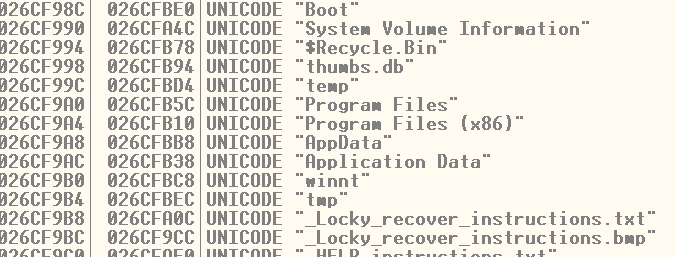
\includegraphics[scale=0.5]{immagini/t2_strings.png}
    \caption{Stringhe caricate dalla \texttt{FUN\_0043c160} per il confronto}
    \label{figura1}
\end{figure}

\vspace{3cm}

\begin{figure}[!h]
    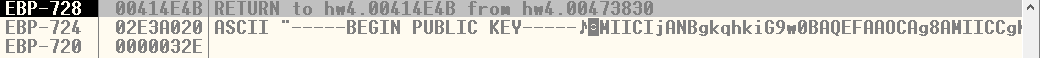
\includegraphics[scale=0.5]{immagini/encr.png}
    \caption{Dati che verranno cifrati nella \texttt{FUN\_00473830}}
    \label{figura2}
\end{figure}

\vspace{3cm}

\begin{figure}[!h]
    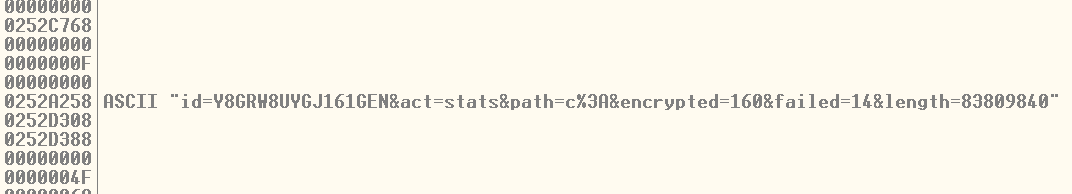
\includegraphics[scale=0.5]{immagini/final_string.png}
    \caption{Possibile stringa riassuntiva del lavoro svolto dal malware}
    \label{figura3}
\end{figure}

\end{document}
